%卒論概要テンプレート ver. 3.0

\documentclass[uplatex,twocolumn,dvipdfmx]{jsarticle}
\usepackage[top=22mm,bottom=22mm,left=22mm,right=22mm]{geometry}
\setlength{\columnsep}{10mm}
\usepackage[T1]{fontenc}
\usepackage{txfonts}
\usepackage[expert,deluxe]{otf}
\usepackage[dvipdfmx,hiresbb]{graphicx}
\usepackage[dvipdfmx]{hyperref}
\usepackage{pxjahyper}
\usepackage{secdot}





%タイトルと学生番号,名前だけ編集すること
\title{\vspace{-5mm}\fontsize{14pt}{0pt}\selectfont 研究タイトル}
\author{\normalsize プロジェクトマネジメントコース 矢吹研究室 1342097 浜野太豪}
\date{}
\pagestyle{empty}
\begin{document}
\fontsize{10.5pt}{\baselineskip}\selectfont
\maketitle





%以下が本文
\section{序論}



\noindent

ドキュメントの検査にプログラムやツールによるサポートが必要である.なぜなら,システム開発の現場では,様々なドキュメントを作成する必要があるからだ.例えばプロジェクト計画書や要件定義書,マニュアルなどがある.このような文書では,読み手に誤解を与えてはいけない.さらに,わかりやすい文書を書くには一定のルールを守る必要がある.短い文で書くこと,正しい表現方法で書くこと,フォーマットを統一することなどである.このようなルールで,大量のドキュメントを人の目によってチェックすることには限界がある.

そこで継続的インテグレーションを活用する方法がある.継続的インテグレーションとは,プログラム全体を常に統合して動く状態にしておくことである.最近では,ビルド(プログラムのコンパイルや自動テスト,アーカイブ化,ソースコードへのタグ付け,実行環境へのデプロイの一連の手順)を自動化するツールが数多くある\cite{1}.

このような継続的インテグレーションで活用されている自動化ツールを用いて,大量のドキュメントをチェックできるツールを構築する.








 



\noindent


\section{目的}
文書チェックを自動的に行うシステムを構築する.文書を提出した際に,自動で文書チェックプログラムが実行され,実行結果の表示,通知を行う.

\section{手法}
研究室ではドキュメントの変更履歴をバージョン管理システムGitHubを用いて行っている.


構築の手法について以下に示す.
\begin{enumerate}
\item 文書チェックプログラムの設定を行う.
\item 自動化ツールの設定を行う.
\item 文章チェックプログラムと自動化ツールとGitHubの連携を行う.

\end{enumerate}

\section{結果}
Githubに課題研究の概要を提出した場合,文書チェックプログラムによって自動的に文書チェックされる.
\noindent
実行結果を以下に示す.
\noindent
%図の挿入
\begin{figure}[h]
\centering
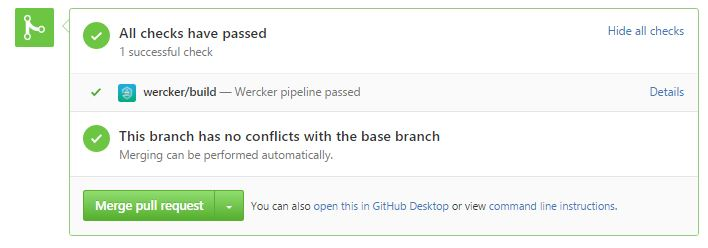
\includegraphics[width=7cm,clip]{3.JPG}
\caption{文書チェックの結果エラーがない場合}\label{}
\end{figure}
%図の挿入
\begin{figure}[h]
\centering
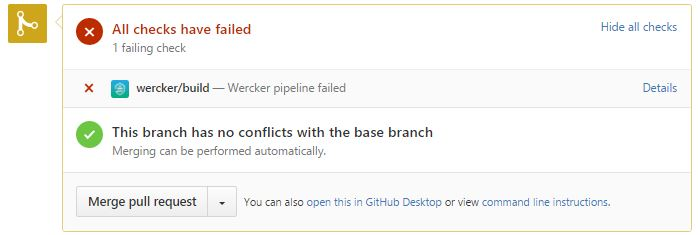
\includegraphics[width=7cm,clip]{2.JPG}
\caption{文書チェックの結果エラーがある場合}\label{}
\end{figure}

\section{考察}
添削済みの課題研究の概要をチェックプログラムにかけてみたところ,数件の指摘が表示された.研究室で運用する場合,文書チェックプログラムの設定の緩和や過去の指摘されやすい部分を重点的に反映させることによって,受け入れやすいものになると考えた.


\section{結論}
自動的に文書チェックを行う環境を構築することができた.文章チェックプログラムの設定の検証を行うことで,研究室で運用可能である.



\bibliographystyle{junsrt}
\bibliography{biblio}%「biblio.bib」というファイルが必要.

\end{document}
